% Created by tikzDevice version 0.12.3.1 on 2023-04-12 14:04:58
% !TEX encoding = UTF-8 Unicode
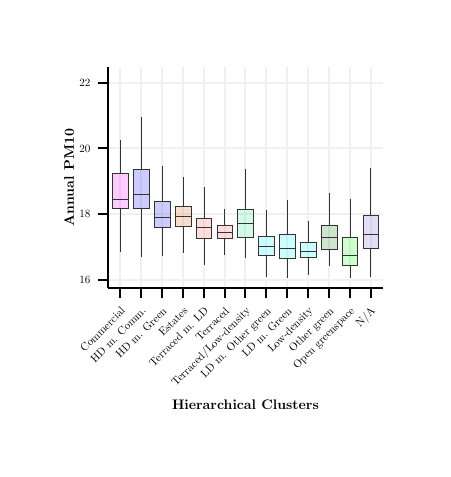
\begin{tikzpicture}[x=1pt,y=1pt]
\definecolor{fillColor}{RGB}{255,255,255}
\path[use as bounding box,fill=fillColor,fill opacity=0.00] (0,0) rectangle (142.64,152.15);
\begin{scope}
\path[clip] (  0.00,  0.00) rectangle (142.64,152.15);
\definecolor{fillColor}{RGB}{255,255,255}

\path[fill=fillColor] (  0.00,  0.00) rectangle (142.64,152.15);
\end{scope}
\begin{scope}
\path[clip] ( 28.95, 58.04) rectangle (128.41,137.92);
\definecolor{fillColor}{RGB}{255,255,255}

\path[fill=fillColor] ( 28.95, 58.04) rectangle (128.41,137.92);
\definecolor{drawColor}{gray}{0.94}

\path[draw=drawColor,line width= 0.7pt,line join=round] ( 28.95, 61.05) --
	(128.41, 61.05);

\path[draw=drawColor,line width= 0.7pt,line join=round] ( 28.95, 84.80) --
	(128.41, 84.80);

\path[draw=drawColor,line width= 0.7pt,line join=round] ( 28.95,108.55) --
	(128.41,108.55);

\path[draw=drawColor,line width= 0.7pt,line join=round] ( 28.95,132.30) --
	(128.41,132.30);

\path[draw=drawColor,line width= 0.7pt,line join=round] ( 33.47, 58.04) --
	( 33.47,137.92);

\path[draw=drawColor,line width= 0.7pt,line join=round] ( 41.00, 58.04) --
	( 41.00,137.92);

\path[draw=drawColor,line width= 0.7pt,line join=round] ( 48.54, 58.04) --
	( 48.54,137.92);

\path[draw=drawColor,line width= 0.7pt,line join=round] ( 56.07, 58.04) --
	( 56.07,137.92);

\path[draw=drawColor,line width= 0.7pt,line join=round] ( 63.61, 58.04) --
	( 63.61,137.92);

\path[draw=drawColor,line width= 0.7pt,line join=round] ( 71.14, 58.04) --
	( 71.14,137.92);

\path[draw=drawColor,line width= 0.7pt,line join=round] ( 78.68, 58.04) --
	( 78.68,137.92);

\path[draw=drawColor,line width= 0.7pt,line join=round] ( 86.21, 58.04) --
	( 86.21,137.92);

\path[draw=drawColor,line width= 0.7pt,line join=round] ( 93.75, 58.04) --
	( 93.75,137.92);

\path[draw=drawColor,line width= 0.7pt,line join=round] (101.29, 58.04) --
	(101.29,137.92);

\path[draw=drawColor,line width= 0.7pt,line join=round] (108.82, 58.04) --
	(108.82,137.92);

\path[draw=drawColor,line width= 0.7pt,line join=round] (116.36, 58.04) --
	(116.36,137.92);

\path[draw=drawColor,line width= 0.7pt,line join=round] (123.89, 58.04) --
	(123.89,137.92);
\definecolor{drawColor}{gray}{0.20}

\path[draw=drawColor,line width= 0.1pt,line join=round] ( 41.00,100.94) -- ( 41.00,119.80);

\path[draw=drawColor,line width= 0.1pt,line join=round] ( 41.00, 87.09) -- ( 41.00, 69.20);
\definecolor{fillColor}{RGB}{0,0,255}

\path[draw=drawColor,line width= 0.1pt,fill=fillColor,fill opacity=0.20] ( 38.18,100.94) --
	( 38.18, 87.09) --
	( 43.83, 87.09) --
	( 43.83,100.94) --
	( 38.18,100.94) --
	cycle;

\path[draw=drawColor,line width= 0.1pt] ( 38.18, 92.15) -- ( 43.83, 92.15);

\path[draw=drawColor,line width= 0.1pt,line join=round] ( 33.47, 99.56) -- ( 33.47,111.42);

\path[draw=drawColor,line width= 0.1pt,line join=round] ( 33.47, 86.87) -- ( 33.47, 71.25);
\definecolor{fillColor}{RGB}{255,0,255}

\path[draw=drawColor,line width= 0.1pt,fill=fillColor,fill opacity=0.20] ( 30.64, 99.56) --
	( 30.64, 86.87) --
	( 36.29, 86.87) --
	( 36.29, 99.56) --
	( 30.64, 99.56) --
	cycle;

\path[draw=drawColor,line width= 0.1pt] ( 30.64, 90.35) -- ( 36.29, 90.35);

\path[draw=drawColor,line width= 0.1pt,line join=round] ( 86.21, 76.69) -- ( 86.21, 86.27);

\path[draw=drawColor,line width= 0.1pt,line join=round] ( 86.21, 70.01) -- ( 86.21, 62.20);
\definecolor{fillColor}{RGB}{0,255,255}

\path[draw=drawColor,line width= 0.1pt,fill=fillColor,fill opacity=0.20] ( 83.39, 76.69) --
	( 83.39, 70.01) --
	( 89.04, 70.01) --
	( 89.04, 76.69) --
	( 83.39, 76.69) --
	cycle;

\path[draw=drawColor,line width= 0.1pt] ( 83.39, 73.09) -- ( 89.04, 73.09);

\path[draw=drawColor,line width= 0.1pt,line join=round] ( 93.75, 77.39) -- ( 93.75, 89.91);

\path[draw=drawColor,line width= 0.1pt,line join=round] ( 93.75, 68.94) -- ( 93.75, 61.67);

\path[draw=drawColor,line width= 0.1pt,fill=fillColor,fill opacity=0.20] ( 90.92, 77.39) --
	( 90.92, 68.94) --
	( 96.58, 68.94) --
	( 96.58, 77.39) --
	( 90.92, 77.39) --
	cycle;

\path[draw=drawColor,line width= 0.1pt] ( 90.92, 72.52) -- ( 96.58, 72.52);

\path[draw=drawColor,line width= 0.1pt,line join=round] (108.82, 80.80) -- (108.82, 92.39);

\path[draw=drawColor,line width= 0.1pt,line join=round] (108.82, 72.10) -- (108.82, 66.17);
\definecolor{fillColor}{RGB}{0,128,0}

\path[draw=drawColor,line width= 0.1pt,fill=fillColor,fill opacity=0.20] (105.99, 80.80) --
	(105.99, 72.10) --
	(111.65, 72.10) --
	(111.65, 80.80) --
	(105.99, 80.80) --
	cycle;

\path[draw=drawColor,line width= 0.1pt] (105.99, 76.32) -- (111.65, 76.32);

\path[draw=drawColor,line width= 0.1pt,line join=round] ( 63.61, 83.48) -- ( 63.61, 94.43);

\path[draw=drawColor,line width= 0.1pt,line join=round] ( 63.61, 76.14) -- ( 63.61, 66.22);
\definecolor{fillColor}{RGB}{255,85,85}

\path[draw=drawColor,line width= 0.1pt,fill=fillColor,fill opacity=0.20] ( 60.78, 83.48) --
	( 60.78, 76.14) --
	( 66.44, 76.14) --
	( 66.44, 83.48) --
	( 60.78, 83.48) --
	cycle;

\path[draw=drawColor,line width= 0.1pt] ( 60.78, 79.97) -- ( 66.44, 79.97);

\path[draw=drawColor,line width= 0.1pt,line join=round] ( 48.54, 89.37) -- ( 48.54,102.03);

\path[draw=drawColor,line width= 0.1pt,line join=round] ( 48.54, 80.23) -- ( 48.54, 69.69);
\definecolor{fillColor}{RGB}{0,0,255}

\path[draw=drawColor,line width= 0.1pt,fill=fillColor,fill opacity=0.20] ( 45.71, 89.37) --
	( 45.71, 80.23) --
	( 51.36, 80.23) --
	( 51.36, 89.37) --
	( 45.71, 89.37) --
	cycle;

\path[draw=drawColor,line width= 0.1pt] ( 45.71, 83.85) -- ( 51.36, 83.85);

\path[draw=drawColor,line width= 0.1pt,line join=round] ( 71.14, 80.94) -- ( 71.14, 86.76);

\path[draw=drawColor,line width= 0.1pt,line join=round] ( 71.14, 76.12) -- ( 71.14, 70.12);
\definecolor{fillColor}{RGB}{255,85,85}

\path[draw=drawColor,line width= 0.1pt,fill=fillColor,fill opacity=0.20] ( 68.32, 80.94) --
	( 68.32, 76.12) --
	( 73.97, 76.12) --
	( 73.97, 80.94) --
	( 68.32, 80.94) --
	cycle;

\path[draw=drawColor,line width= 0.1pt] ( 68.32, 78.41) -- ( 73.97, 78.41);

\path[draw=drawColor,line width= 0.1pt,line join=round] (101.29, 74.51) -- (101.29, 82.22);

\path[draw=drawColor,line width= 0.1pt,line join=round] (101.29, 69.35) -- (101.29, 62.77);
\definecolor{fillColor}{RGB}{0,255,255}

\path[draw=drawColor,line width= 0.1pt,fill=fillColor,fill opacity=0.20] ( 98.46, 74.51) --
	( 98.46, 69.35) --
	(104.11, 69.35) --
	(104.11, 74.51) --
	( 98.46, 74.51) --
	cycle;

\path[draw=drawColor,line width= 0.1pt] ( 98.46, 71.52) -- (104.11, 71.52);

\path[draw=drawColor,line width= 0.1pt,line join=round] ( 78.68, 86.53) -- ( 78.68,101.05);

\path[draw=drawColor,line width= 0.1pt,line join=round] ( 78.68, 76.44) -- ( 78.68, 68.97);
\definecolor{fillColor}{RGB}{37,229,137}

\path[draw=drawColor,line width= 0.1pt,fill=fillColor,fill opacity=0.20] ( 75.85, 86.53) --
	( 75.85, 76.44) --
	( 81.51, 76.44) --
	( 81.51, 86.53) --
	( 75.85, 86.53) --
	cycle;

\path[draw=drawColor,line width= 0.1pt] ( 75.85, 81.46) -- ( 81.51, 81.46);

\path[draw=drawColor,line width= 0.1pt,line join=round] (116.36, 76.32) -- (116.36, 90.32);

\path[draw=drawColor,line width= 0.1pt,line join=round] (116.36, 66.31) -- (116.36, 61.83);
\definecolor{fillColor}{RGB}{0,255,0}

\path[draw=drawColor,line width= 0.1pt,fill=fillColor,fill opacity=0.20] (113.53, 76.32) --
	(113.53, 66.31) --
	(119.18, 66.31) --
	(119.18, 76.32) --
	(113.53, 76.32) --
	cycle;

\path[draw=drawColor,line width= 0.1pt] (113.53, 69.91) -- (119.18, 69.91);

\path[draw=drawColor,line width= 0.1pt,line join=round] ( 56.07, 87.75) -- ( 56.07, 98.23);

\path[draw=drawColor,line width= 0.1pt,line join=round] ( 56.07, 80.30) -- ( 56.07, 70.60);
\definecolor{fillColor}{RGB}{212,85,0}

\path[draw=drawColor,line width= 0.1pt,fill=fillColor,fill opacity=0.20] ( 53.25, 87.75) --
	( 53.25, 80.30) --
	( 58.90, 80.30) --
	( 58.90, 87.75) --
	( 53.25, 87.75) --
	cycle;

\path[draw=drawColor,line width= 0.1pt] ( 53.25, 83.98) -- ( 58.90, 83.98);

\path[draw=drawColor,line width= 0.1pt,line join=round] (123.89, 84.23) -- (123.89,101.53);

\path[draw=drawColor,line width= 0.1pt,line join=round] (123.89, 72.57) -- (123.89, 61.95);
\definecolor{fillColor}{RGB}{106,90,205}

\path[draw=drawColor,line width= 0.1pt,fill=fillColor,fill opacity=0.20] (121.07, 84.23) --
	(121.07, 72.57) --
	(126.72, 72.57) --
	(126.72, 84.23) --
	(121.07, 84.23) --
	cycle;

\path[draw=drawColor,line width= 0.1pt] (121.07, 77.40) -- (126.72, 77.40);

\path[] ( 28.95, 58.04) rectangle (128.41,137.92);
\end{scope}
\begin{scope}
\path[clip] (  0.00,  0.00) rectangle (142.64,152.15);
\definecolor{drawColor}{RGB}{0,0,0}

\path[draw=drawColor,line width= 0.7pt,line join=round] ( 28.95, 58.04) --
	( 28.95,137.92);
\end{scope}
\begin{scope}
\path[clip] (  0.00,  0.00) rectangle (142.64,152.15);
\definecolor{drawColor}{RGB}{0,0,0}

\node[text=drawColor,anchor=base east,inner sep=0pt, outer sep=0pt, scale=  0.40] at ( 22.65, 59.67) {16};

\node[text=drawColor,anchor=base east,inner sep=0pt, outer sep=0pt, scale=  0.40] at ( 22.65, 83.42) {18};

\node[text=drawColor,anchor=base east,inner sep=0pt, outer sep=0pt, scale=  0.40] at ( 22.65,107.17) {20};

\node[text=drawColor,anchor=base east,inner sep=0pt, outer sep=0pt, scale=  0.40] at ( 22.65,130.92) {22};
\end{scope}
\begin{scope}
\path[clip] (  0.00,  0.00) rectangle (142.64,152.15);
\definecolor{drawColor}{RGB}{0,0,0}

\path[draw=drawColor,line width= 0.7pt,line join=round] ( 25.45, 61.05) --
	( 28.95, 61.05);

\path[draw=drawColor,line width= 0.7pt,line join=round] ( 25.45, 84.80) --
	( 28.95, 84.80);

\path[draw=drawColor,line width= 0.7pt,line join=round] ( 25.45,108.55) --
	( 28.95,108.55);

\path[draw=drawColor,line width= 0.7pt,line join=round] ( 25.45,132.30) --
	( 28.95,132.30);
\end{scope}
\begin{scope}
\path[clip] (  0.00,  0.00) rectangle (142.64,152.15);
\definecolor{drawColor}{RGB}{0,0,0}

\path[draw=drawColor,line width= 0.7pt,line join=round] ( 28.95, 58.04) --
	(128.41, 58.04);
\end{scope}
\begin{scope}
\path[clip] (  0.00,  0.00) rectangle (142.64,152.15);
\definecolor{drawColor}{RGB}{0,0,0}

\path[draw=drawColor,line width= 0.7pt,line join=round] ( 33.47, 54.54) --
	( 33.47, 58.04);

\path[draw=drawColor,line width= 0.7pt,line join=round] ( 41.00, 54.54) --
	( 41.00, 58.04);

\path[draw=drawColor,line width= 0.7pt,line join=round] ( 48.54, 54.54) --
	( 48.54, 58.04);

\path[draw=drawColor,line width= 0.7pt,line join=round] ( 56.07, 54.54) --
	( 56.07, 58.04);

\path[draw=drawColor,line width= 0.7pt,line join=round] ( 63.61, 54.54) --
	( 63.61, 58.04);

\path[draw=drawColor,line width= 0.7pt,line join=round] ( 71.14, 54.54) --
	( 71.14, 58.04);

\path[draw=drawColor,line width= 0.7pt,line join=round] ( 78.68, 54.54) --
	( 78.68, 58.04);

\path[draw=drawColor,line width= 0.7pt,line join=round] ( 86.21, 54.54) --
	( 86.21, 58.04);

\path[draw=drawColor,line width= 0.7pt,line join=round] ( 93.75, 54.54) --
	( 93.75, 58.04);

\path[draw=drawColor,line width= 0.7pt,line join=round] (101.29, 54.54) --
	(101.29, 58.04);

\path[draw=drawColor,line width= 0.7pt,line join=round] (108.82, 54.54) --
	(108.82, 58.04);

\path[draw=drawColor,line width= 0.7pt,line join=round] (116.36, 54.54) --
	(116.36, 58.04);

\path[draw=drawColor,line width= 0.7pt,line join=round] (123.89, 54.54) --
	(123.89, 58.04);
\end{scope}
\begin{scope}
\path[clip] (  0.00,  0.00) rectangle (142.64,152.15);
\definecolor{drawColor}{RGB}{0,0,0}

\node[text=drawColor,rotate= 45.00,anchor=base east,inner sep=0pt, outer sep=0pt, scale=  0.40] at ( 35.40, 49.51) {Commercial};

\node[text=drawColor,rotate= 45.00,anchor=base east,inner sep=0pt, outer sep=0pt, scale=  0.40] at ( 42.93, 49.51) {HD m. Comm.};

\node[text=drawColor,rotate= 45.00,anchor=base east,inner sep=0pt, outer sep=0pt, scale=  0.40] at ( 50.47, 49.51) {HD m. Green};

\node[text=drawColor,rotate= 45.00,anchor=base east,inner sep=0pt, outer sep=0pt, scale=  0.40] at ( 58.00, 49.51) {Estates};

\node[text=drawColor,rotate= 45.00,anchor=base east,inner sep=0pt, outer sep=0pt, scale=  0.40] at ( 65.54, 49.51) {Terraced m. LD};

\node[text=drawColor,rotate= 45.00,anchor=base east,inner sep=0pt, outer sep=0pt, scale=  0.40] at ( 73.07, 49.51) {Terraced};

\node[text=drawColor,rotate= 45.00,anchor=base east,inner sep=0pt, outer sep=0pt, scale=  0.40] at ( 80.61, 49.51) {Terraced/Low-density};

\node[text=drawColor,rotate= 45.00,anchor=base east,inner sep=0pt, outer sep=0pt, scale=  0.40] at ( 88.14, 49.51) {LD m. Other green};

\node[text=drawColor,rotate= 45.00,anchor=base east,inner sep=0pt, outer sep=0pt, scale=  0.40] at ( 95.68, 49.51) {LD m. Green};

\node[text=drawColor,rotate= 45.00,anchor=base east,inner sep=0pt, outer sep=0pt, scale=  0.40] at (103.21, 49.51) {Low-density};

\node[text=drawColor,rotate= 45.00,anchor=base east,inner sep=0pt, outer sep=0pt, scale=  0.40] at (110.75, 49.51) {Other green};

\node[text=drawColor,rotate= 45.00,anchor=base east,inner sep=0pt, outer sep=0pt, scale=  0.40] at (118.28, 49.51) {Open greenspace};

\node[text=drawColor,rotate= 45.00,anchor=base east,inner sep=0pt, outer sep=0pt, scale=  0.40] at (125.82, 49.51) {N/A};
\end{scope}
\begin{scope}
\path[clip] (  0.00,  0.00) rectangle (142.64,152.15);
\definecolor{drawColor}{RGB}{0,0,0}

\node[text=drawColor,anchor=base,inner sep=0pt, outer sep=0pt, scale=  0.50] at ( 78.68, 14.03) {\bfseries Hierarchical Clusters};
\end{scope}
\begin{scope}
\path[clip] (  0.00,  0.00) rectangle (142.64,152.15);
\definecolor{drawColor}{RGB}{0,0,0}

\node[text=drawColor,rotate= 90.00,anchor=base,inner sep=0pt, outer sep=0pt, scale=  0.50] at ( 16.70, 97.98) {\bfseries Annual PM10};
\end{scope}
\end{tikzpicture}
